\textbf{{1.链路状态协议}}

如果要算路由器1到路由器2、3、4的最短路径(给出邻接矩阵,即链路状态数据库),就可以将路由器1看成是起始结点,然后使用3次Dijkstra算法分别计算出路由器1到路由器2、3、4的最短路径,路由表就出来了。一旦网络拓扑又有变化,如以前没有相连的路由器,现在相连了,就又按照这样的步骤去计算路由表,这就是链路状态协议。

\textbf{{2. OSPF协议介绍}}

{为了使OSPF路由协议能够用于规模很大的网络,并且使其收敛得更快,OSPF路由协议将一个自治系统再划分为若干个更小的范围,称为\textbf{区域},如下图所示。}

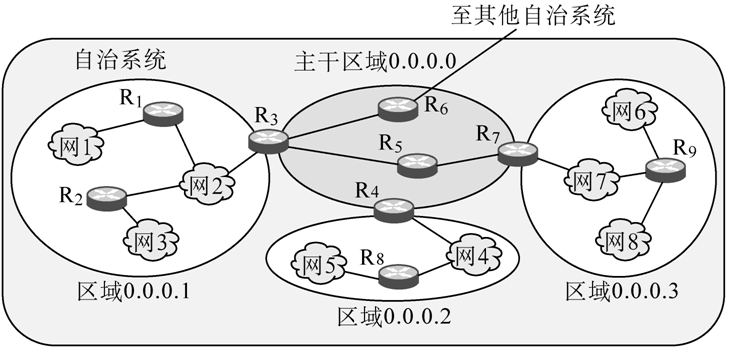
\includegraphics[width=3.12500in,height=1.51042in]{png-jpeg-pics/2E13E707A209CCB2E953519FE7AECD56.png}

\textbf{\textbf{{3. OSPF协议三要点}}}

1)向本自治系统中所有路由器发送信息,这里使用的方法是{\textbf{洪泛法}}。

2)发送的信息就是\textbf{与本路由器相邻的所有路由器的链路状态},但这只是路由器所知道的部分信息。

3)``链路状态''就是说明本路由器都和哪些路由器相邻以及该链路的``度量''(metric)。

{\textbf{注意:}{\textbf{只有当链路状态发生变化时},路由器才用洪泛法向所有路由器发送此信息。}}

\textbf{{4.OSPF的5种分组类型}}

\textbf{1)}类型1。问候(Hello)分组,用来发现和维持邻站的可达性;

\textbf{2)}类型2。数据库描述分组,向邻站给出自己的链路状态数据库中的所有链路状态项目的摘要信息;

\textbf{3)}类型3。链路状态请求分组,向对方请求发送某些链路项目的详细信息;

\textbf{4)}类型4。链路状态更新分组,用洪泛法对全网更新链路状态;

\textbf{5)}类型5。链路状态确认分组,对链路更新分组的确认。
